% Slides for 2025-08-12
% To create a slide, use the following:
% \begin{frame}{TITLE}
%     BODY
% \end{frame}

% To create a slide with a bullet list, use the following:
% \begin{frame}{TITLE}
%     \begin{itemize}
%         \item ITEM 1
%         \item ITEM 2
%     \end{itemize}    
% \end{frame}

% To create a slide with numbered list, use the following:
% \begin{frame}{TITLE}
%     \begin{enumerate}
%         \item ITEM 1
%         \item ITEM 2
%     \end{enumerate}
% \end{frame}

% To create a slide with a graphic:
% 1. Add the graphic to this folder (named picture.png)
% 2. Use the following:
% \begin{frame}{TITLE}
%     \centering
%     \includegraphics[height=0.7\textheight,width=0.7\textwidth,keepaspectratio]{picture.png}
% \end{frame}

% To create a slide with two columns, use the following:
% \begin{frame}{TITLE}
%     \begin{columns}
%         \begin{column}{0.5\textwidth}
%             COLUMN 1 BODY
%         \end{column}
%         \begin{column}{0.5\textwidth}
%             COLUMN 2 BODY
%         \end{column}
%     \end{columns}
% \end{frame}

\begin{frame}{DWE on Rubik Pi}
     \begin{enumerate}
        \item Picture of Rubik Pi with DWE and maybe some results?
    \end{enumerate}
    % \centering
    % \includegraphics[height=0.7\textheight,width=0.7\textwidth,keepaspectratio]{picture.png}
\end{frame}

\begin{frame}{GPU Acceleration Setup on Rubik Pi}
   \begin{itemize}
       \item \textbf{Challenge:} Rubik Pi+ Debian 13 lacking Adreno GPU userland drivers
       \item \textbf{Solution:} Ubuntu chroot environment 
       \item \textbf{Implementation:}
           \begin{itemize}
               \item Configured OpenCL and Vulkan for Adreno GPU support
               \item Built diagnostic tools (\texttt{clinfo}, \texttt{vulkaninfo}) from source
           \end{itemize}
       \item \textbf{Next Step:} Benchmarking GPU performance
   \end{itemize}
   % \centering
   % \includegraphics[height=0.4\textheight,width=0.7\textwidth,keepaspectratio]{}
\end{frame}

\begin{frame}{TITLE}
    \begin{columns}
        \begin{column}{0.5\textwidth}
            \includegraphics[height=0.7\textheight,width=0.3\textwidth,keepaspectratio]{picture.png}
        \end{column}
        \begin{column}{0.5\textwidth}
            \includegraphics[height=0.7\textheight,width=0.3\textwidth,keepaspectratio]{picture.png}
        \end{column}
    \end{columns}
\end{frame}

\begin{frame}{Fishy Data}
    \begin{columns}
        \begin{column}{0.5\textwidth}
            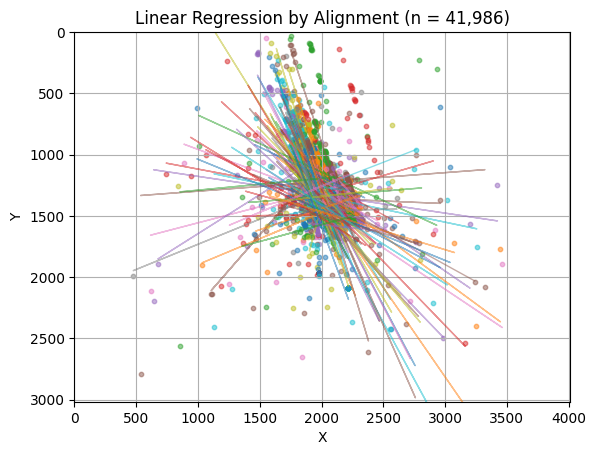
\includegraphics[width=\linewidth,keepaspectratio]{weekly_presentations/images/regression.png}
        \end{column}
        \begin{column}{0.5\textwidth}
            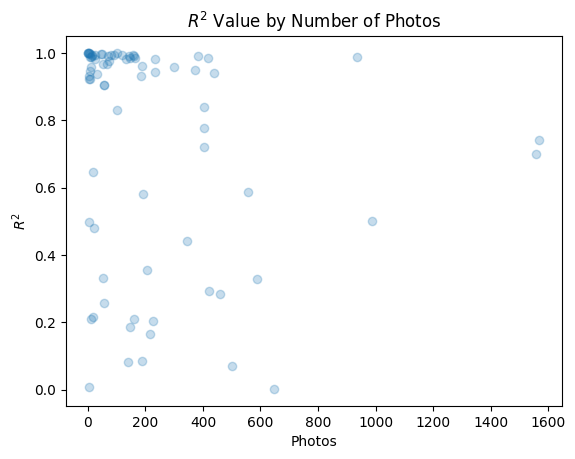
\includegraphics[width=\linewidth,keepaspectratio]{weekly_presentations/images/rsquare.png}
        \end{column}
    \end{columns}

    \vspace{0.2em} % adjust space above the text
    \begin{center}
        {\small Cutoff $R^2\geq 0.9$ and number of photos $\geq 10$ yields 5592}
    \end{center}
\end{frame}

\begin{frame}{Sensing Fish}
    \begin{columns}
        \begin{column}{0.33\textwidth}
            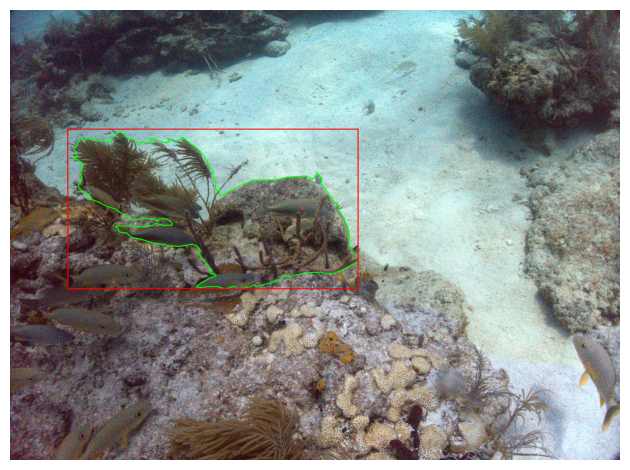
\includegraphics[width=\linewidth,keepaspectratio]{weekly_presentations/images/original.png}
            \caption{Default}
        \end{column}
        \begin{column}{0.33\textwidth}
            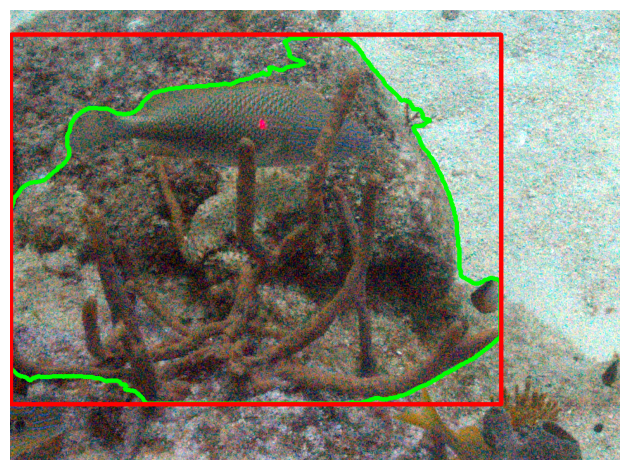
\includegraphics[width=\linewidth,keepaspectratio]{weekly_presentations/images/current.png}
            \caption{Current}
        \end{column}
        \begin{column}{0.33\textwidth}
            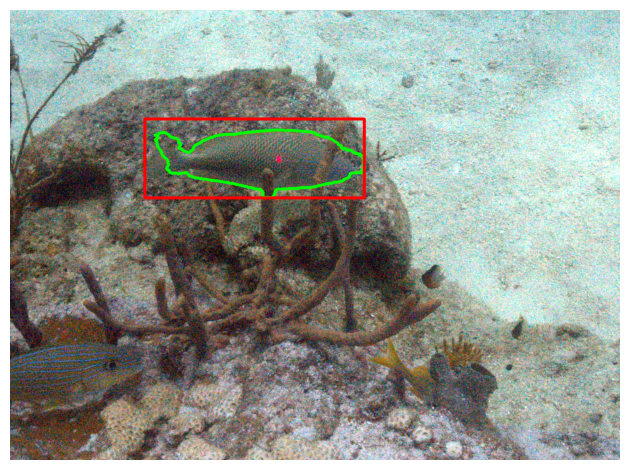
\includegraphics[width=\linewidth,keepaspectratio]{weekly_presentations/images/ideal.png}
            \caption{Goal}
        \end{column}
        
    \end{columns}

\end{frame}
